%! TEX root = 'main.tex'
\section{Evaluation}
\label{sec:implant-evaluation}

In this section, we evaluated several aspects of \name. Since it is a hardware backdoor, we need to measure its physical dimensions and appearance. We also evaluated the effects of \name on the PLC, including the impacts on the performance, memory storage, and power consumption.

The model PLC is the Allen Bradley 1769-L18ER-BBIB CompactLogix
5370, which is equipped with a TI Stellaris LM3S2793 microcontroller. The microcontroller is based on ARM Cortex-M3 architecture and operates at 80MHz. It has 128KB single-cycle flash memory and 64KB single-cycle SRAM. The PLC has 16 DC digital inputs and 16 DC digital outputs, which eventually corresponds to the microcontroller's GPIO port.

\texttt{\textbf{Dimensions and appearance.}} We use commercial off-the-shelf modules to build the prototype, namely the Teensy 3.2 development board and Waveshare SIM800C HAT. They are not the smallest in size. For example,  the SIM800C in SiP packaging with a minimal PCB board is much smaller. However, the SiP needs a voltage of 3.7 volts which a Lithium-Ion battery usually provides. GSM is an impulse type transmitting power, even though the average current is low, but the instantaneous current can reach more than 1.5A, so the board's external power supply is necessary. 

\begin{figure}[h]
	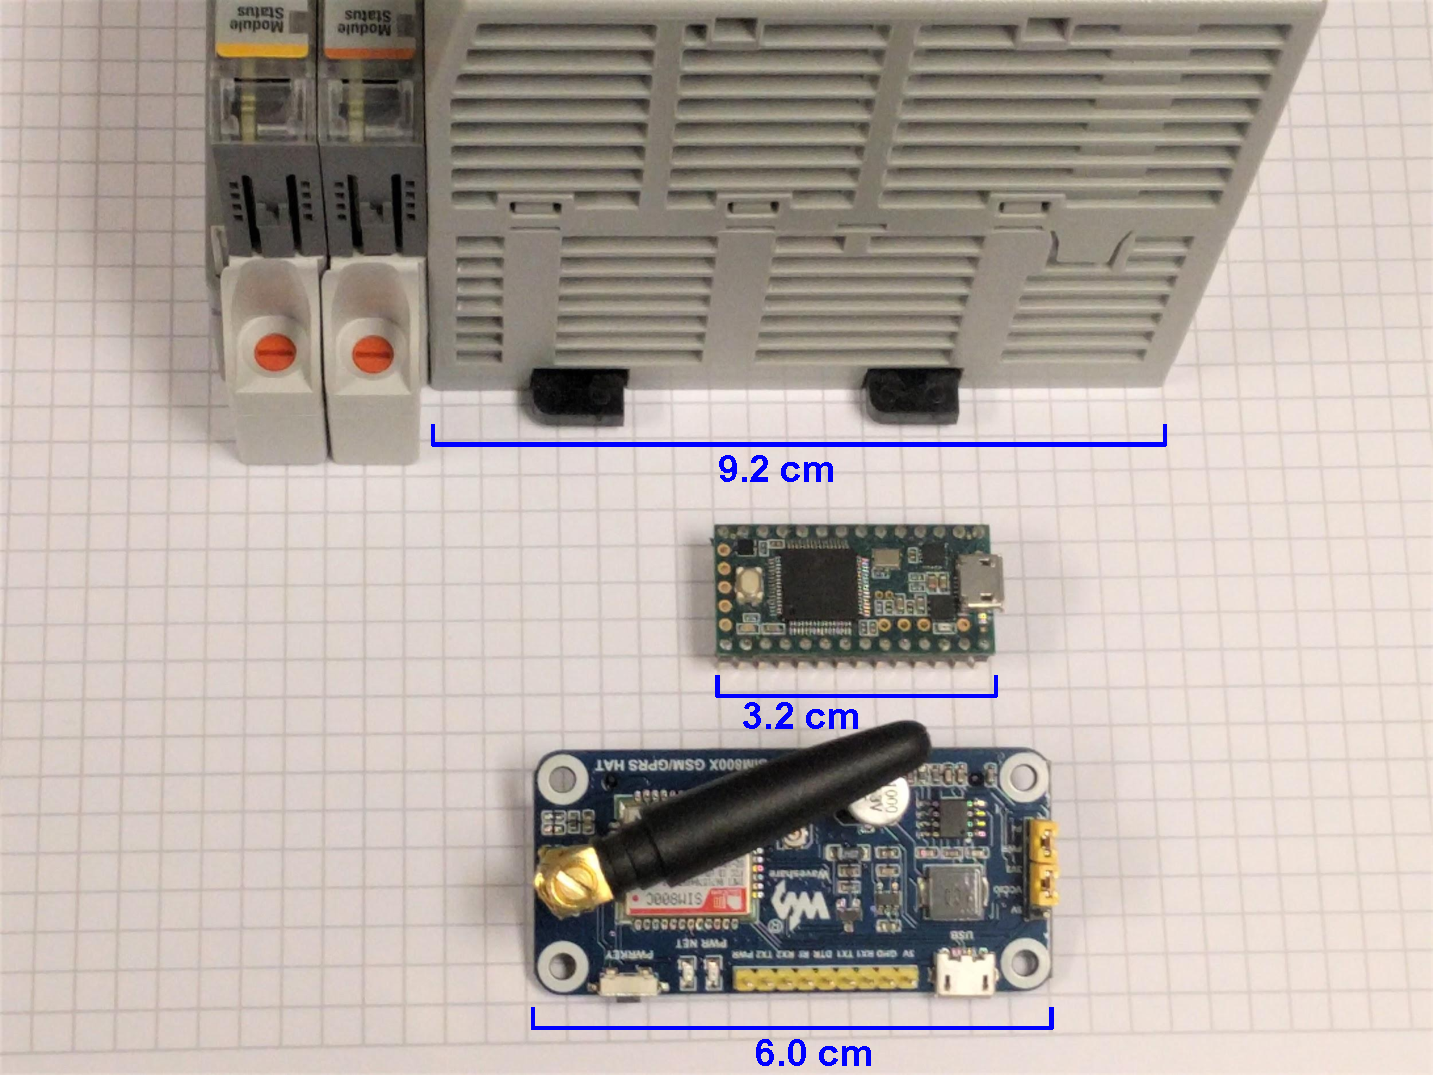
\includegraphics[width=0.47\textwidth]{figures/eval_size}
	\centering
	\caption{The Allen Bradley 1769-L18ER-BBIB CompactLogix
	5370 PLC is in a 9.2cm x 13cm rectangle shape with sufficient space to contain the two bords and extra wires and connectors. The SIM800C HAT takes a full-size sim card, and the antenna takes much space.}
	\label{fig:eval_size}
\end{figure}

~\autoref{fig:eval_size} shows the physical size of the two boards compared to the Allen Bradley PLC. Notice that the two main chips on each board are relatively small. Especially some WIFI chips~\cite{babiuch2019using}~\cite{artenstein2017broadpwn} also provide a microcontroller for general-purpose tasks, which the two chips can combine.  In that case, the hardware can further reduce its size. However, we can not shrink its physical size as small as invisible.  We argue that the more effective way to hide the hardware implant is to make it easily overlooked. It means to use customed PCB with the same color and same style connector attaching to the PLC's board. Because until today, there is very little information publicly available regarding those widely deployed PLCs.  Some good examples are the separate IPMI (Intelligent Platform Management Interface)~\cite{slaight2003using} and KVM (Board, Video, and Mouse)~\cite{kedziorek2007hpc} modules that usually mounted on the server's motherboards.

\begin{figure}[h]
	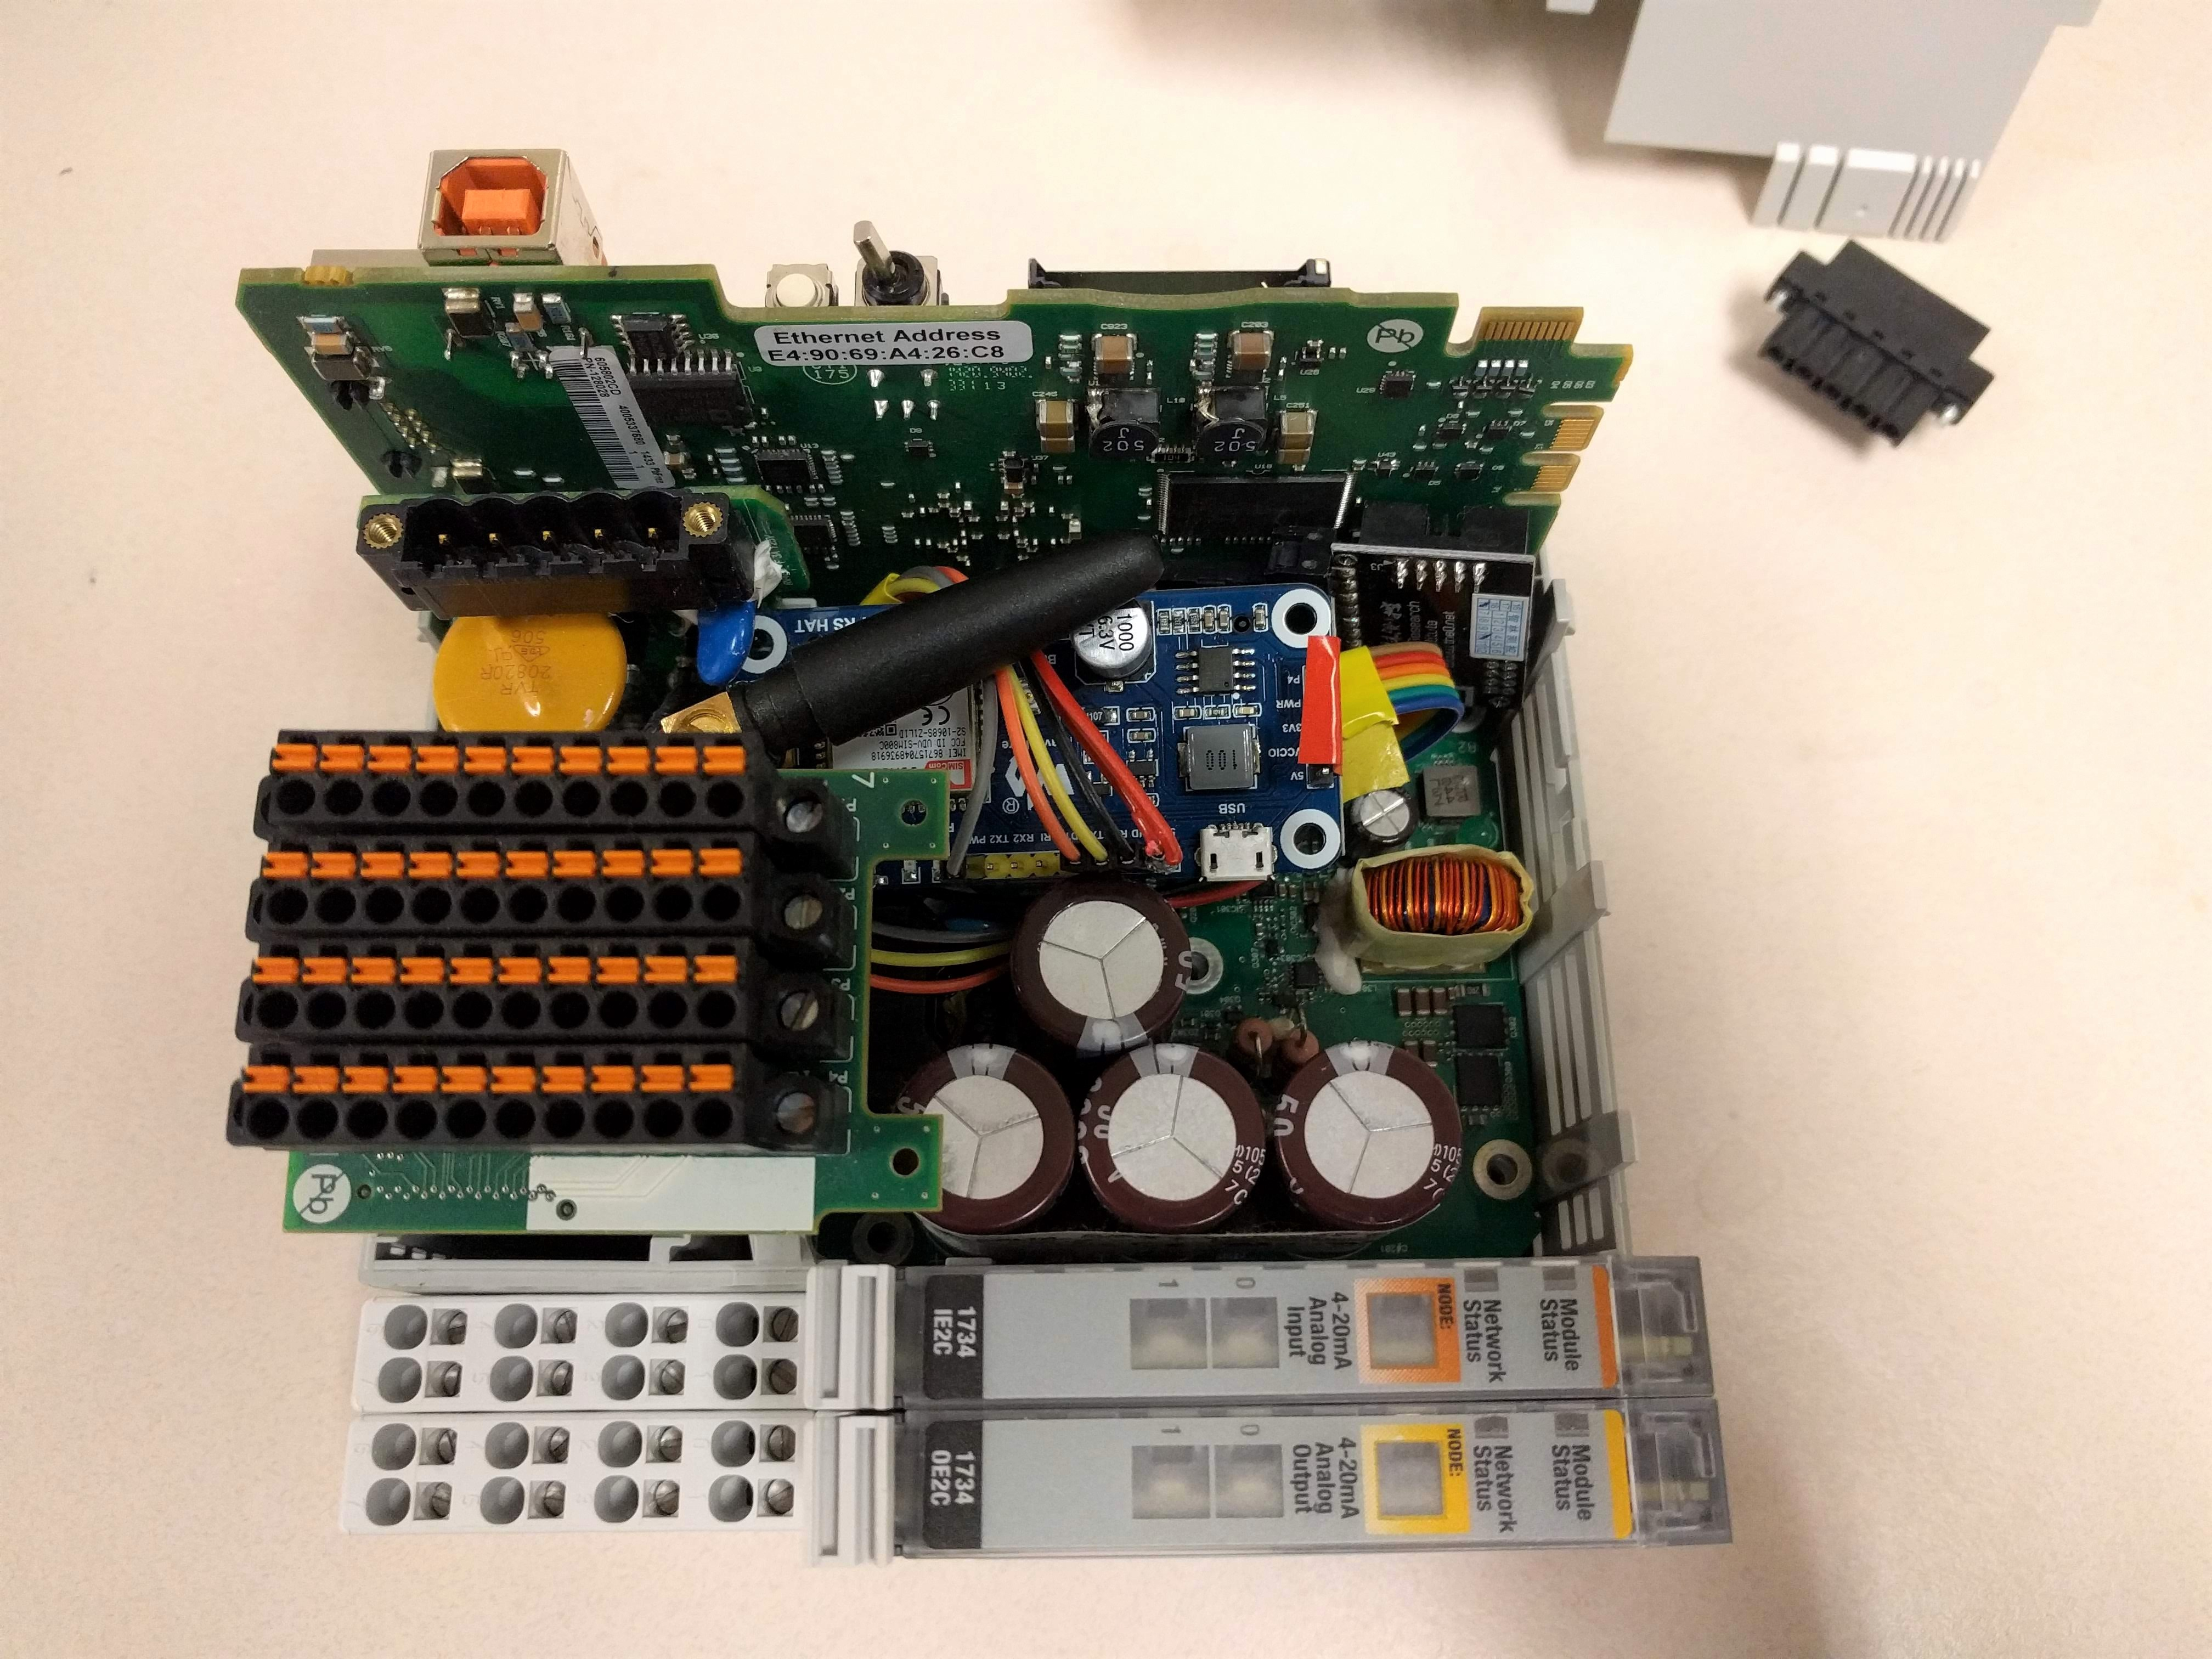
\includegraphics[width=0.47\textwidth]{figures/eval_a}
	\centering
	\caption{We cover the necessary parts using tape to prevent a short circuit. The \name connects to the PLC's microcontroller board's JTAG pad through a 10-pin socket and a long cable. The antenna for receiving GSM signal is also stuffed inside the PLC.}
	\label{fig:eval_a}
\end{figure}

\begin{figure*}[t]
	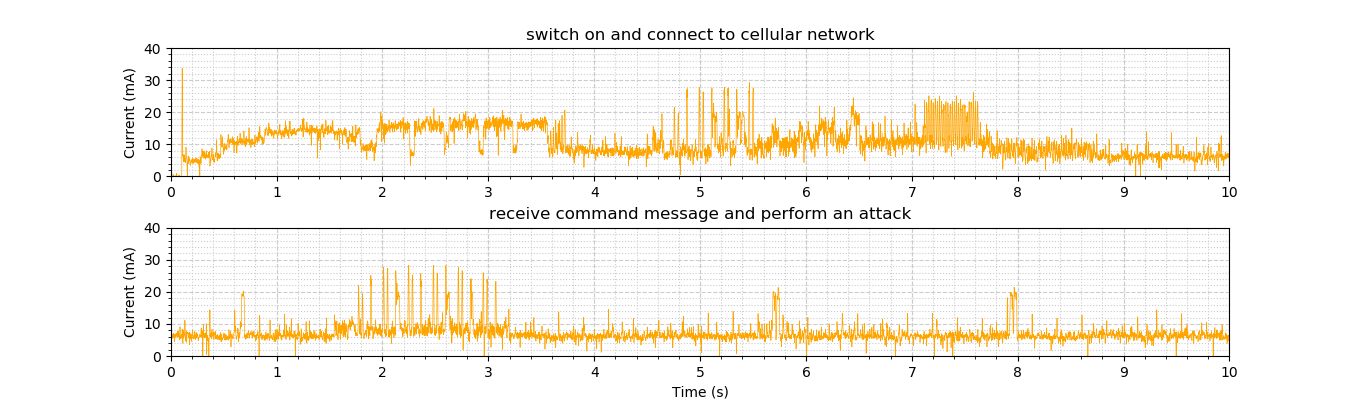
\includegraphics[width=\textwidth]{figures/current}
	\centering
	\caption{The hardware implant does not consume a lot of power, and the power consumption will only increase slightly when starting and executing the attack command. Sub-figure 1 shows the power consumption during the startup. Sub-figure 2.a shows the power consumption during an demo attack. 2.b indicates an output pin of the attacked PLC. }
	\label{fig:current}
\end{figure*}

~\autoref{fig:eval_a} shows that after wiring two boards and wrapping them with tape to prevent a short circuit, it is small enough to fit inside the PLC's plastic case. We connect the JTAG pads with GPIO pins from the Teensy board. One of the PLC we use for this experiment turns out to have a 10-pin socket soldered on the pad, but all other PLCs we own do not have such a setting. A novel design for easy installation avoiding soldering in the field and reliable connection with the JTAG pad is necessary. We consider this as one of our further works.

\begin{figure}[h]
	\centering
    \begin{subfigure}[b]{0.22\textwidth}
    	\centering
	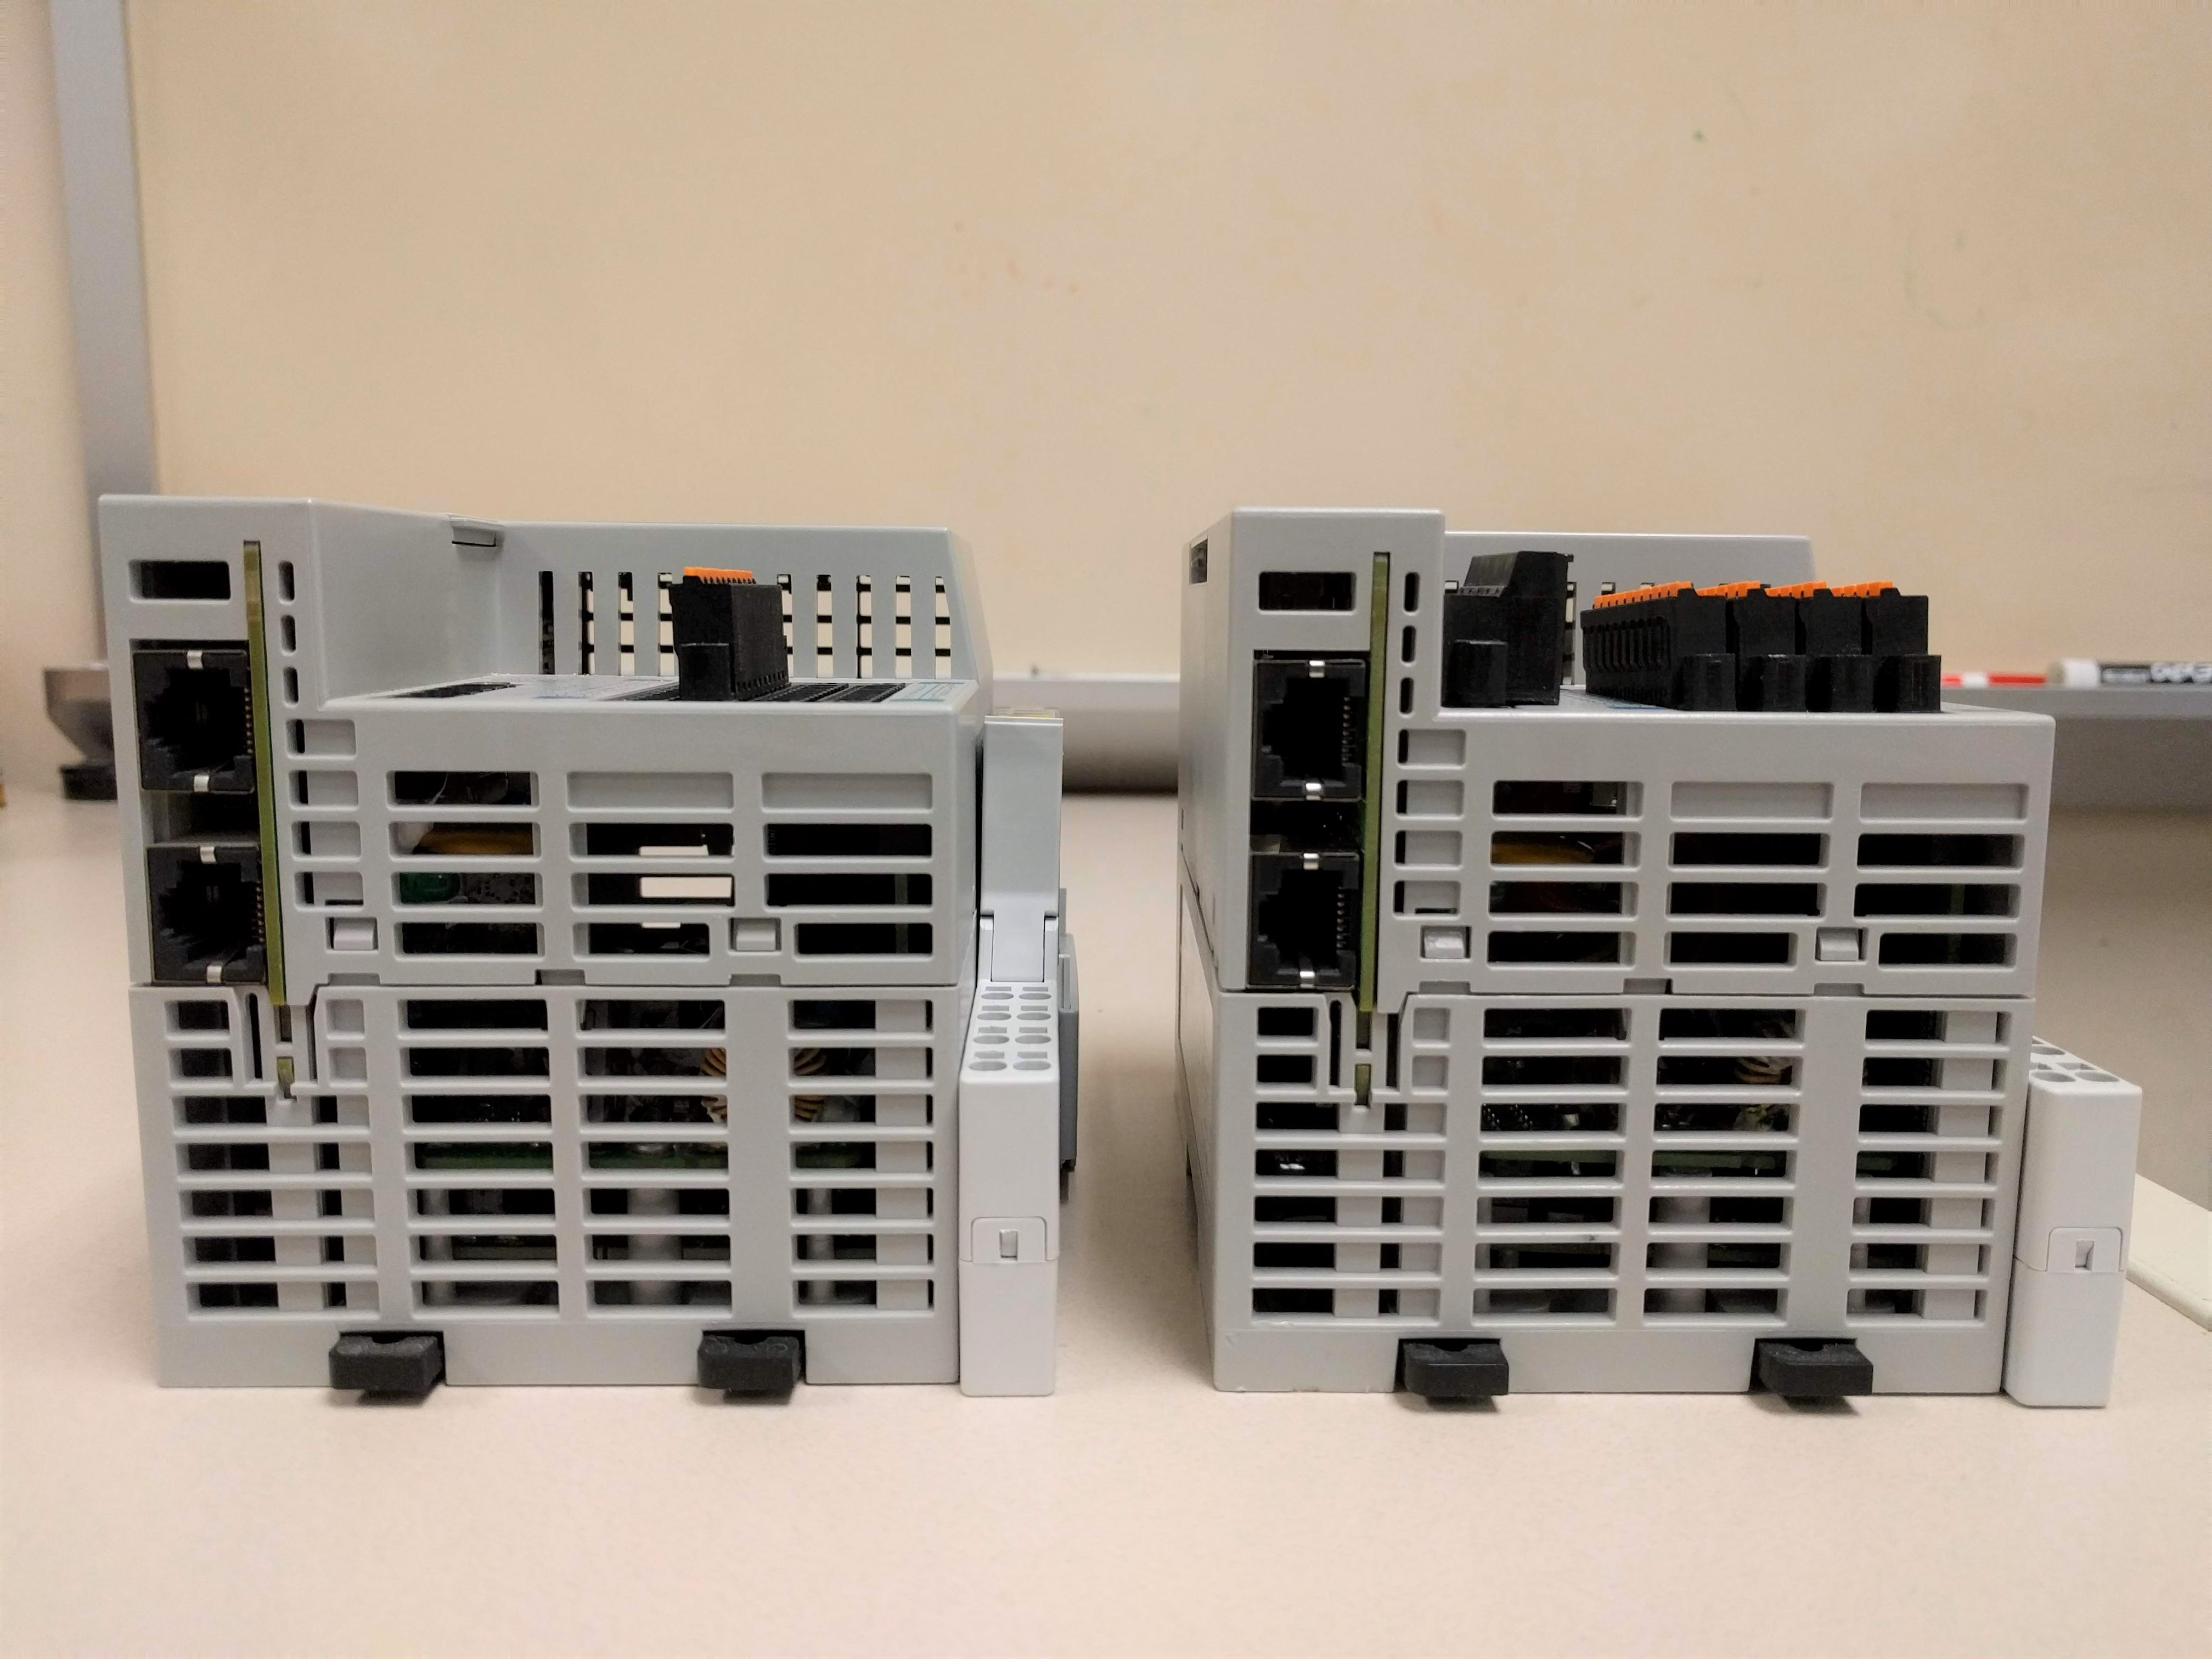
\includegraphics[width=1\textwidth]{figures/eval_b2}
        \vspace{-0.15in}
        \caption{Front}
		\label{fig:eval_b1}
	\end{subfigure}
%~\qquad
	\begin{subfigure}[b]{0.22\textwidth}
    	\centering
	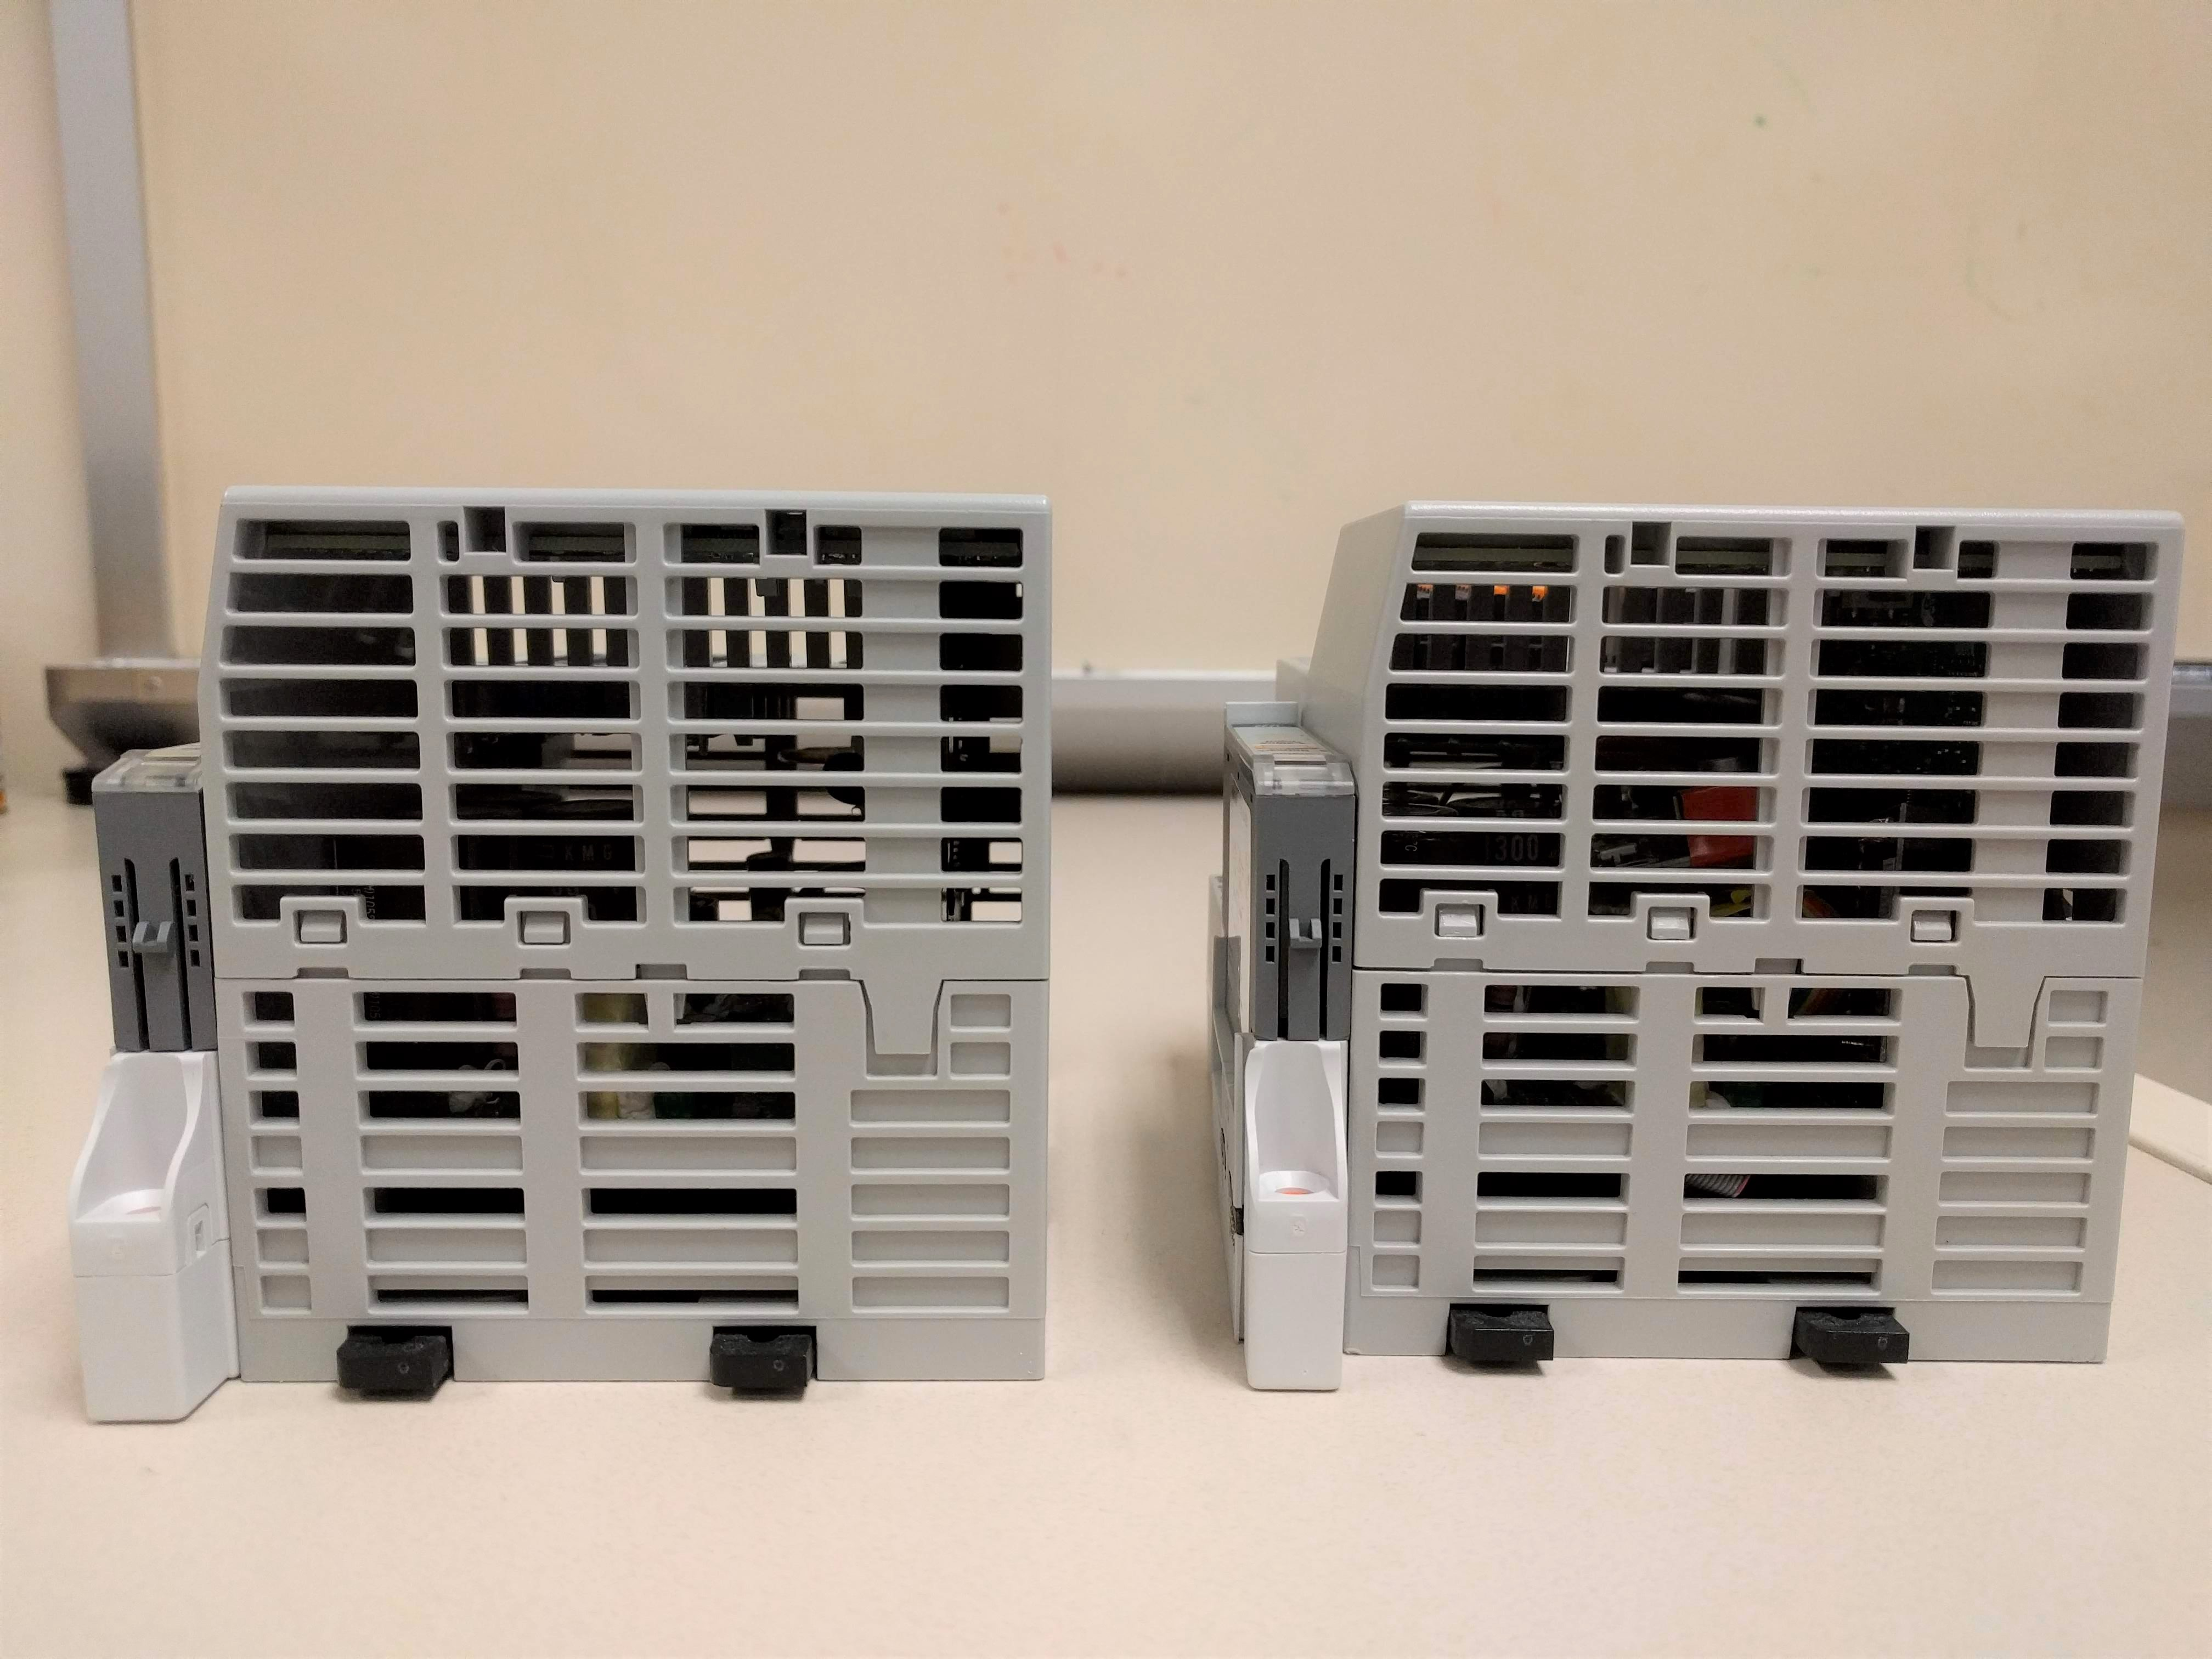
\includegraphics[width=1\textwidth]{figures/eval_b1}
        \vspace{-0.15in}
	\caption{Back}
		\label{fig:eval_b2}
	\end{subfigure}
    \vspace{-0.15in}
    \caption{The two figures are the Allen Bradley 1769-L18ER-BBIB CompactLogix 5370 PLC's front and back view, in which both the PLC on the right has the hardware implant installed. There is no significant difference from the appearance point of view, and no parts are exposed to the outside.}
		\label{fig:eval_b}
	\vspace{-0.15in}
\end{figure}

As shown in~\autoref{fig:eval_b}, the hardware implant is not noticeable from the PLC's outside appearance; no parts are exposed, it only seems to take up some space. However, heat dissipation may be a problem to be considered in the future.


\texttt{\textbf{Performance.}} Since this backdoor is implemented on the hardware level, it almost cost zero performance overhead. For instance, if we choose to change IO through override signals transmitting in the low-speed bus, pull-up or pull-down the voltage level, there will be no overhead added to the microcontroller. On the other side, if we use the JTAG interface instead, it may cause a slight performance overhead based on the microarchitecture. Due to various implementations, JTAG debugging capabilities can be intrusive or non-intrusive. The conventional JTAG debug is invasive, which halt the processor using breakpoints and watchpoints. It also needs to halt the processor before it can modify any register.

Nevertheless, the debug functionality provided in LM3S2793 is as CoreSight components. It provides real-time access for the debugger without halting the processor to AMBA system memory, peripheral registers, and all debug configuration registers. Therefore \name can modify the GPIO through the AHB bus without any software overhead.

Also, the external or timer interrupt may be delayed for a few clock cycles when encountering JTAG related operations. However, \name has no operation when in standby mode, and controls on IO only take a few memory reads/writes. Furthermore, we regulate our attacking operations at a low pace not to jam the system.  The resulting performance overhead is generally negligible, as shown in~\autoref{fig:exetime}.

\begin{figure}[h]
	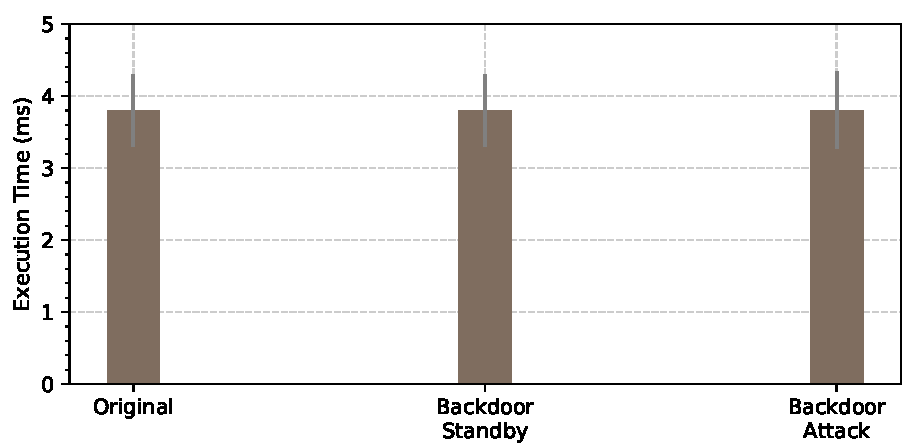
\includegraphics[width=0.47\textwidth]{figures/exetime}
	\centering
	\caption{To accumulate execution time, we use a counter in the ladder logic and use an output signal to indicate the begin/end time of the test. During the standby test, \name has attached the PLC, but no command is sent. We alter the PLC's output every 500ms to imitate a malicious operation for the attack test.}
	\label{fig:exetime}
\end{figure}

\texttt{\textbf{Memory Consumption.}} \name neither occupies flash memory to reside on the system nor take SRAM during the runtime. Even when it is controlling IO, the operations are performed on memory-mapped IO for GPIO ports. Therefore, the memory consumption for \name is zero.



\texttt{\textbf{Power Consumption.}}  Because of the extra circuitry we bring to the system,  the power consumption of the PLC increases. Although the two embedded devices consume very little power compared to the field power that the PLC provides, this is an anomaly we brought into the system. Therefore we measure it with the PLC that is connected to the field power but carries no applicants. We connect a resistor in series to the power supply line of the PLC and use an oscilloscope to measure the voltage across the resistor. \autoref{fig:current} shows that several slight current peaks occur when the cellular chip is searching and connecting to the GSM network and when \name receives the SMS message and sending JTAG commands to the PLC.



%\subsection{Performance}
%
%In our threat model, this hardware implant should exist independently of the PLC's communication network. To achieve this, as mentioned before, we chose to use cellular networks to communicate with nodes via SMS message. This approach is not as reliable as wired networks, especially in our attack model, which may require multiple nodes to launch attacks at the same time. We evaluated the approximate time required for SMS transmission, as shown in~\autoref{fig:smstime}, although we know that this may be affected by a variety of factors, such as the distance between the cell phone and the base station, the number of cell phones served by the same base station, across different networks, and so on. We also know that a SMS message over 160 characters will be split, large messages are segmented into 153 character segments and sent individually then rebuilt by the recipients device. But in order to avoid differences in the protocols implemented by different SMS programs or there may be some extra bytes attached to the SMS message, we did not strictly evaluate it by the number of SMS segments. From a practical point of view, we evaluated the transmission time corresponding to the length of the control command.


\texttt{\textbf{SMS Message.}} One concern we have is that since the antenna is also stuff inside the PLC's case, the signal strength may not be good. So we test it for receiving various lengths of SMS messages, as shown in ~\autoref{fig:smstime}. We use a phone to send the command messages to \name, and we send each command 20 times to calculate the average. The cellular networks we used are T-Mobile and Google Fi. Although the time of message transmission is not very accurate, it is reliable. Different lengths of information have different purposes. For starting a denial-of-service attack or a pre-defined function, one byte is enough. To change specific IO, we need a few bytes to descript its address or index. We also test receiving hundreds of bytes. It can be used to update the firmware on the PLC's flash remotely.

\begin{figure}[th]
	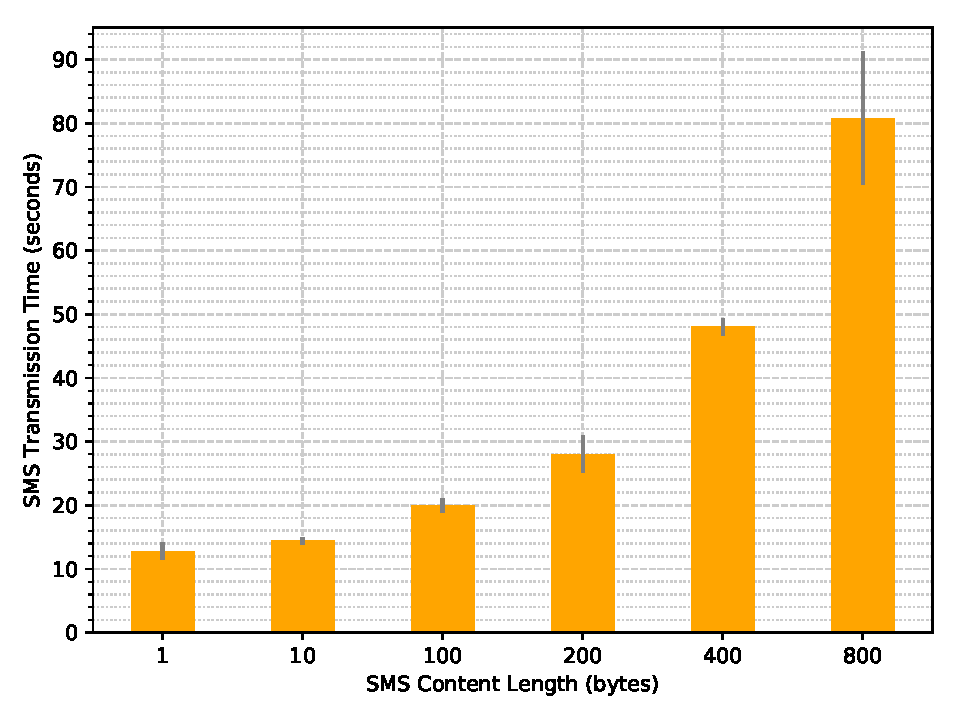
\includegraphics[width=0.47\textwidth]{figures/smstime}
	\centering
	\caption{SMS Message Transmission Time}
	\label{fig:smstime}
\end{figure}

%The control command length can be only one byte, which is used to start a malicious function preset in the hardware implant. It can also be very long, such as containing a piece of binary to update the firmware of the PLC. Or it can contain a series of detailed attack instructions. The advantage of this is that even if the hardware implant is exposed, it does not contain specific attack instructions, thus avoiding further exposure to subsequence attacks and methods.
%
%We get the data by sending a control command to a node with a phone. The command for each length was tested 20 times to obtain the mean and standard deviation. The cellular networks we used is T-Mobile and Google Fi. 
%
%As shown in the figure, the longer the length of the control command, the more time it takes, and the less reliable it is for an attack that requires precise synchronization.
%
%Since the payload (attack commands) is either pre-existing in the hardware implant or sent by the command message during the attack. The attack in our instance directly manipulates the output of the GPIO. So it does not need to modify any code in any PLC firmware, nor does it need to occupy the storage space of the PLC.
%
%Due to different implementations, JTAG debugging capabilities can be intrusive or non-intrusive. The conventional JTAG debug is invasive which halt the processor using breakpoints and watchpoints. It also needs to halt the processor before it can modify any register. However, the debug functionality implemented in LM3S2793 is known as CoreSight architecture. The DAP (Debug Access Port) is an implementation of an ARM Debug Interface which provides real-time access for the debugger without halting the processor to AMBA system memory, peripheral registers and all debug configuration registers. So our hardware implant can modify the GPIO through AHB bus without any software overhead.
%

%The hardware implant is powered directly from the PLC and does not consume a lot of power. The power consumption will only increase slightly when starting and executing the attack command, as shown in~\autoref{fig:current}.






